\documentclass{article}
\usepackage[utf8]{inputenc}
%\usepackage{natbib}
\usepackage{graphicx}
\usepackage[hidelinks]{hyperref}
\usepackage{color}
\usepackage{listings}
%\usepackage{lastpage}
\usepackage{wrapfig}
%\usepackage{eso-pic}
%\usepackage{tikz}
\usepackage{float}
\usepackage{amssymb}
\usepackage{caption}
\usepackage{subcaption}
%\usepackage{pdfpages}
\usepackage[backend=biber]{biblatex}
\definecolor{commentgreen}{RGB}{100, 190, 100}
\definecolor{gray}{RGB}{50, 50, 50}
\lstset{language=C,
                breaklines=true,
                basicstyle=\ttfamily\scriptsize,
                keywordstyle=\color{blue}\ttfamily,
                stringstyle=\color{red}\ttfamily,
                commentstyle=\color{commentgreen}\ttfamily,
                morecomment=[l][\color{magenta}]{\#},
                numberstyle=\tiny\color{gray},
                numbers=left
}


\title{CGP - Mini-project:\\Water Shader}
\author{Jannick Drews}
\date{\today}

\newcommand{\secref}[1]{\nameref{#1}~\ref{#1}}
\newcommand{\goodcite}[1]{\textsuperscript{\cite{#1}}}

\addbibresource{Ref.bib}

\setlength\parindent{0pt}
\begin{document}
\pagenumbering{gobble}
\maketitle
\newpage
\pagenumbering{arabic}

%% For this mini-project, you have to create and showcase an advanced shader and talk about the theory behind it. 
%% You should be able to depict a deep understanding of your code, to be able to explain how it works and how you 
%%  overcome the technical challenges you met.  Such shader can be, but not limited to: %% list of suggestions here%%
%%

\section{Abstract}
\label{sec:abstract}


\section{Introduction}
\label{sec:introduction}
A water shader can be built in many different ways, this report will cover how I developed my shader, the challenges I faced and how I reached my goals. To start with I was looking for a unique way to develop the water shader, usually the shader is made using a bump or normal map for the water itself, in this project I was aiming for using voronoi as the bump map.

\section{Theory}
\label{sec:theory}
This section will cover all theory related to the shader. This will include; Voronoi, bump maps, reflections and refractions, fragment and vertex knowledge, fresnel effect, transparency, culling, z-buffer and grabpass.

\subsection{Fragment \& Vertex}
\label{sec:frag_vert}
The \textbf{fragment} and \textbf{vertex} shaders are both shaders but they work in different spaces. The vertex shader works on the local space, object space and afterwards converts the space to the clip space. The fragment shader works by modifying the mesh on the clip space, which will finally be convert to screen space.


\subsection{Voronoi}
\label{sec:voronoi}
The voronoi effect is made by having, typically a grid of 9 cells which each have a random point, and from that point a distance is calculated to each other cell. Depending on that distance, each pixel will be colored with less and less saturation. You could argue that it is a radial colouration that happens, colouring outwards from the center point.\\

\begin{figure}[H]
    \centering
    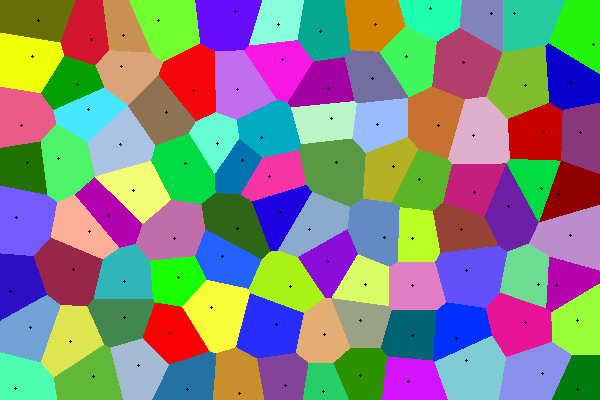
\includegraphics[width=.75\textwidth]{img/voronoi}
    \caption{Voronoi\protect\footnotemark}
    \label{fig:voronoi}
\end{figure}
\footnotetext{\url{https://www.codeproject.com/KB/recipes/882739/Fig_1.png}}
\autoref{fig:voronoi} shows the voronoi effect. Each cell is uniquely coloured to better showcase the effect, the voronoi effect is usually coupled with a time variable with a sinus or cosinus function applied to make each cell move with time passed.\\

I've used this effect on the vertex shader, applying it in object space as to generate a bump map which I utilize to visualize the waves on the object. The voronoi affect is applied via the normals of the mesh.
% UI scaling etc

\subsection{Bump maps}
\label{sec:bump_map}
Bump maps in shaders is utilized by having a greyscale image or texture tell where the object should modify the verteces positions. Ergo translating the position of the verteces to a new position after shader application. This can be applied to either the vertex or fragment shader respectively.

\subsection{Reflections \& Refraction}
\label{sec:refl_refr}

\subsubsection{Grabpass}
\label{sec:grabpass}

\subsection{Fresnel effect}
\label{sec:fresnel_effect}
The Fresnel effect is blablabla..\\It can be used to visualize reflective objects color, when viewed at a critical angle. The effect is a bright surface, which will form around the object, no matter the camera angle, and is applied in clipspace.
%\begin{figure}[H]
%    \centering
%    \includegraphics[width=.75\textwidth]{img/fresnel}
%    \caption{Voronoi\protect\footnotemark}
%    \label{fig:voronoi}
%\end{figure}



% Voronoi
% Bump map
% Reflection & Refraction(distort)
% Additive color
% Local space & clip space
% Fragment & vertex shader
% Fresnel
% Transparency & the NON usage of it
% Culling
% z-buffer
% grabpass

\section{Description \& Analysis}
\label{sec:descript_n_analysis}
% Screenshots
\begin{figure}[H]
    \centering
    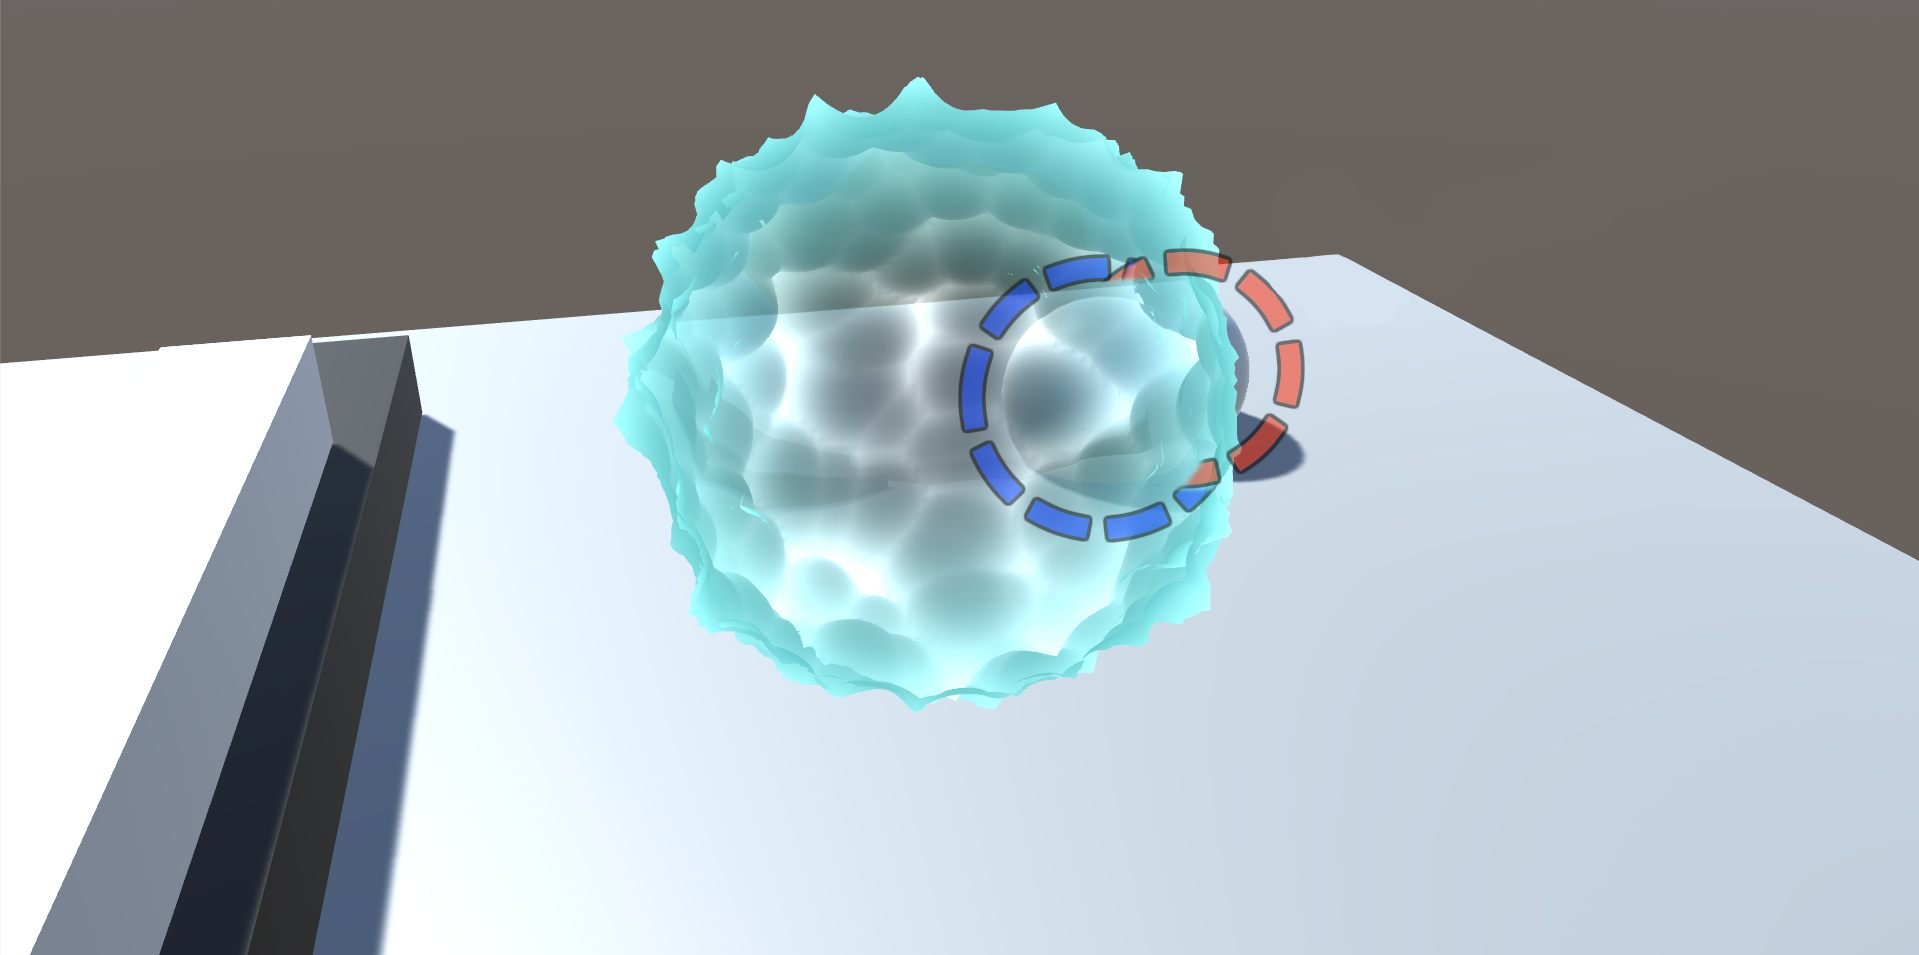
\includegraphics[width=\textwidth]{img/shader_1_guide_v2}
    \caption{Shader - Refraction illustration}
    \label{fig:shader_1}
\end{figure}
\autoref{fig:shader_1} shows a capture of the scene with the shader applied to a sphere. The effect of the Grabpass can be seen as a substitude for refraction, see \secref{sec:refl_refr} \& \secref{sec:grabpass}.\\

The red indicator on the figure shows the original real position of a sphere which is placed behind the object with the shader applied. The blue indicators denote the distortion of the image with the new location of the object being refracted.\\Technically, the shader does not have any transparent properties, instead a Grabpass is used which is discussed in \secref{sec:grabpass}.\\

This gives a better refraction of the object(subjective), compared to when cubemap refractions are used. Since cubemaps require an object to be in a static position in space or constantly update a cubemap image, the grabpass is a faster and more "headache free" alternative.\\


\begin{figure}[H]
    \centering
    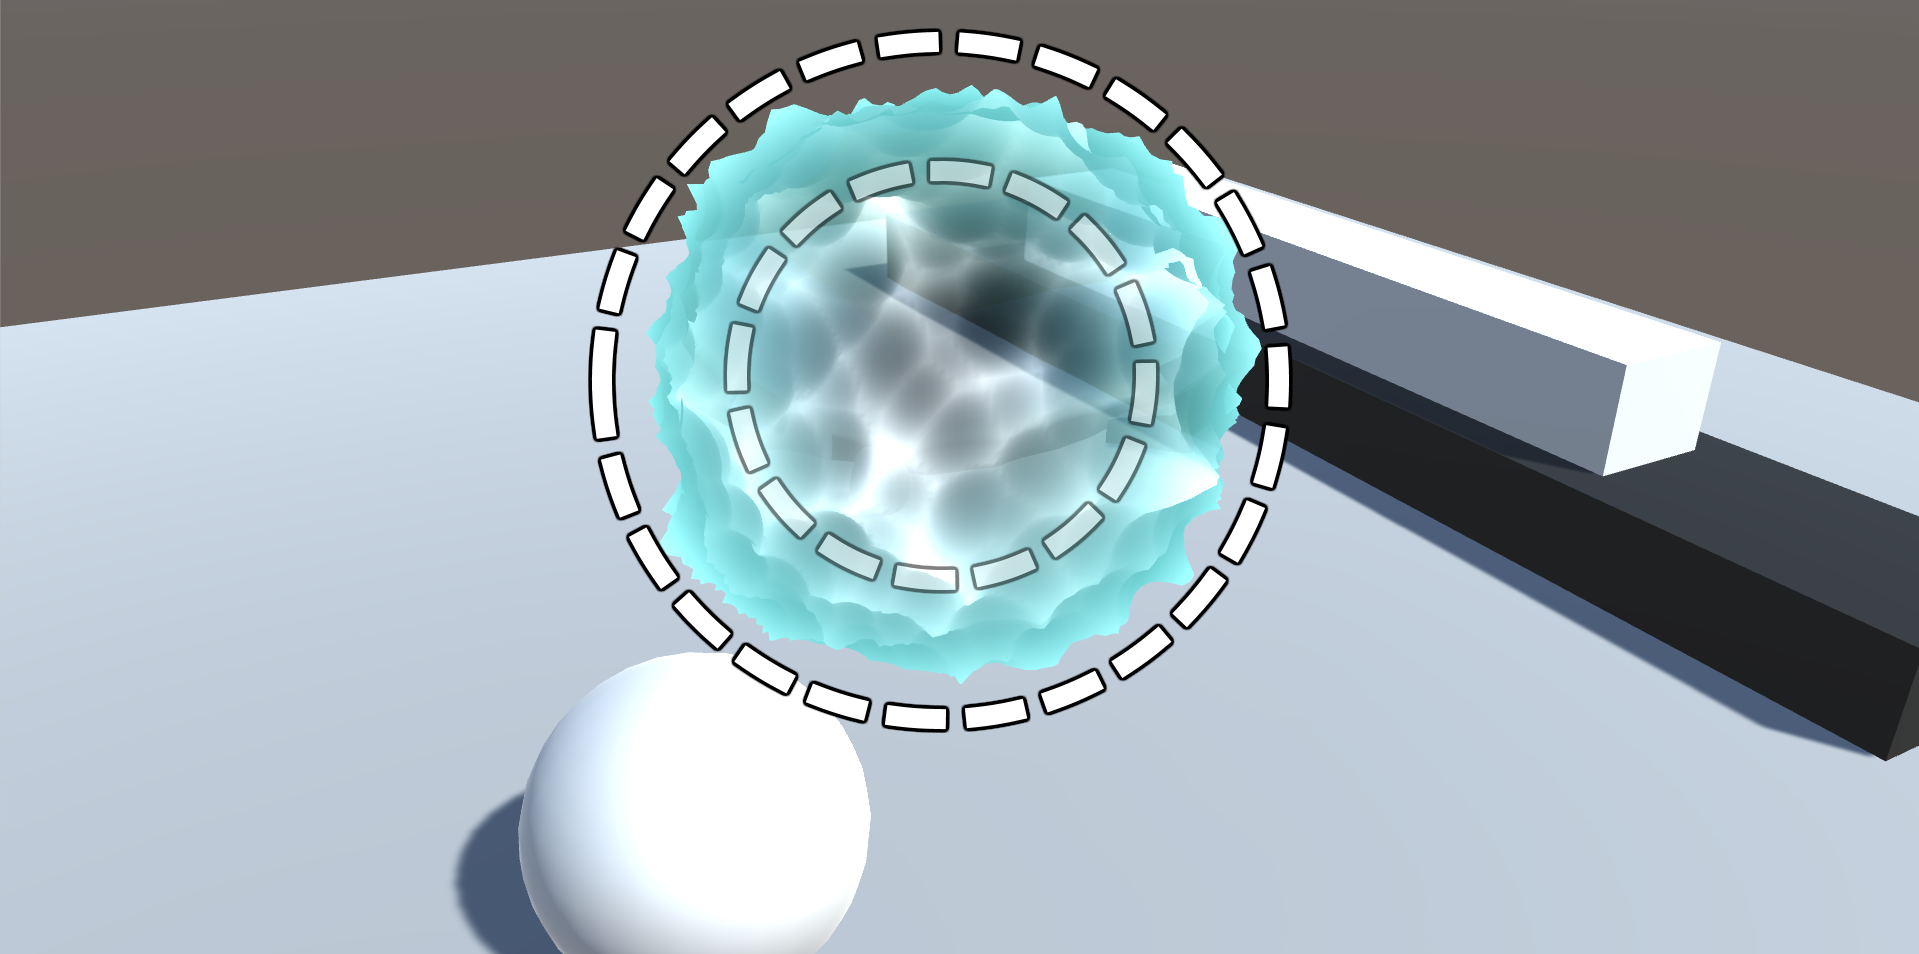
\includegraphics[width=\textwidth]{img/shader_2}
    \caption{Shader, fresnel effect and additive bumpmap}
    \label{fig:shader_2}
\end{figure}
\autoref{fig:shader_2} shows the fresnel effect with some added extra colours from the pre-defined color of the shader and the voronoi bump map colors.

\begin{figure}[H]
    \centering
    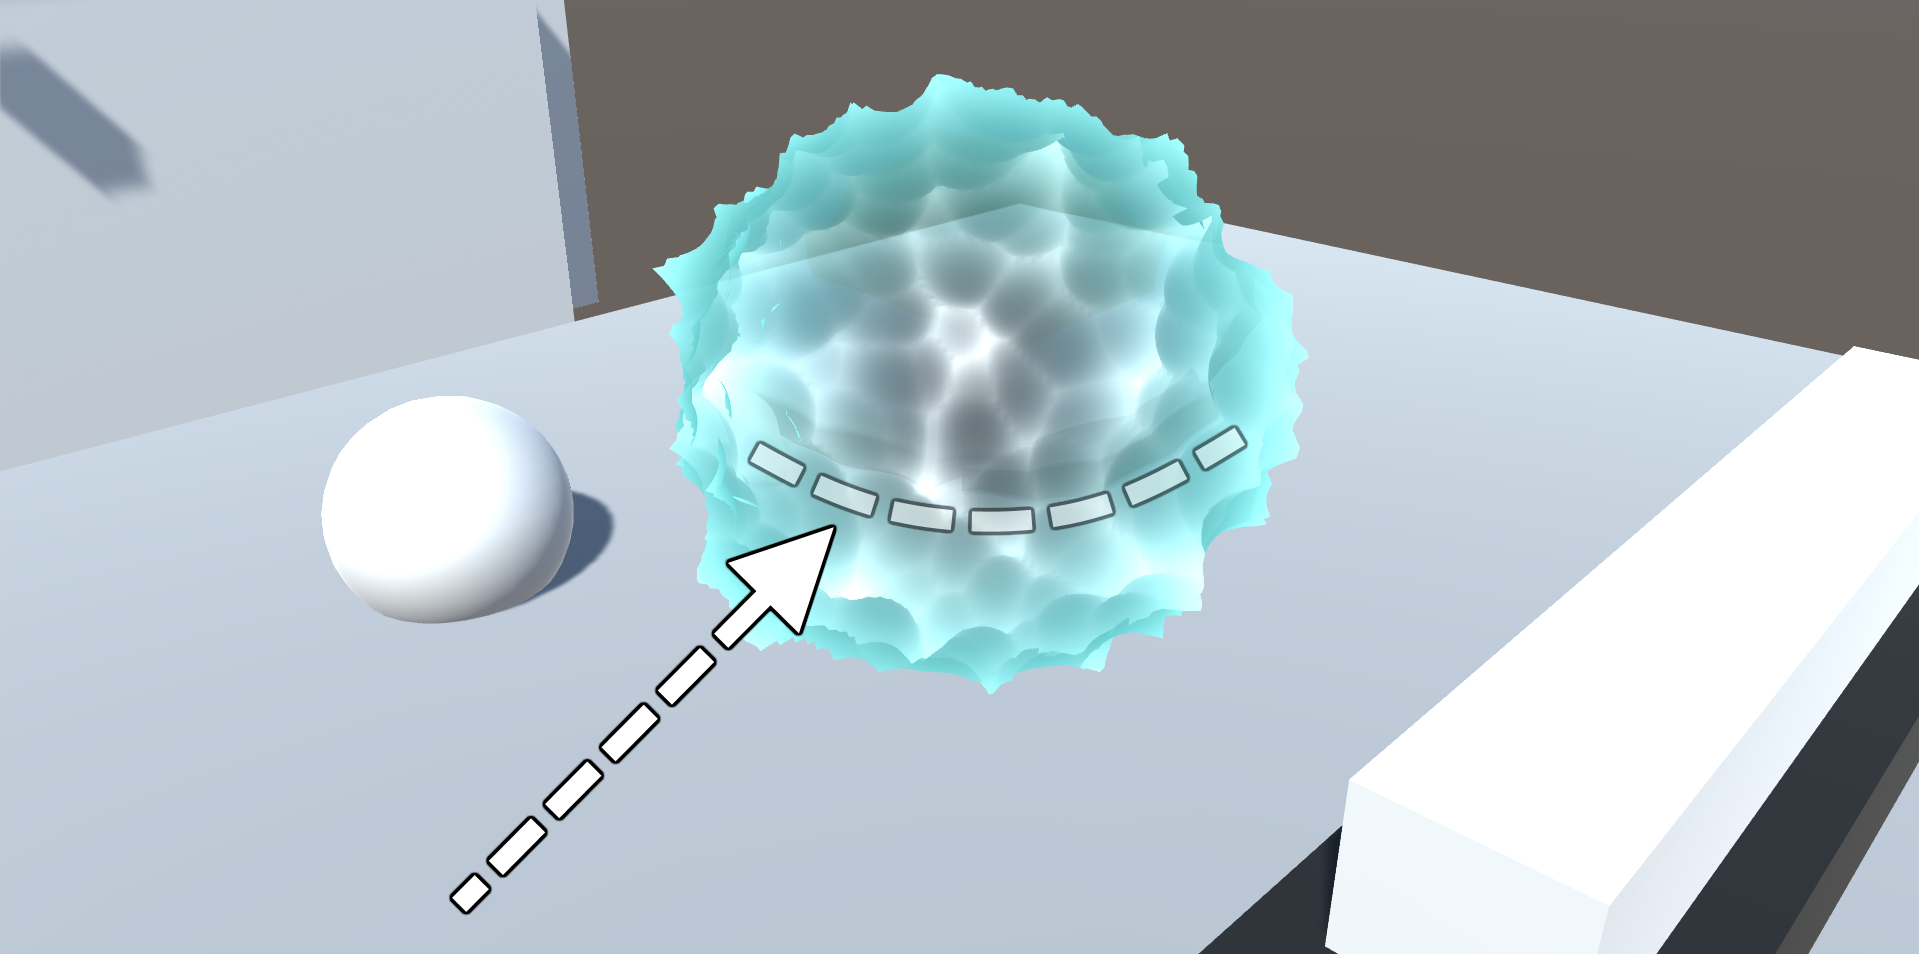
\includegraphics[width=\textwidth]{img/shader_3}
    \caption{Shader}
    \label{fig:shader_3}
\end{figure}
\begin{figure}[H]
    \centering
    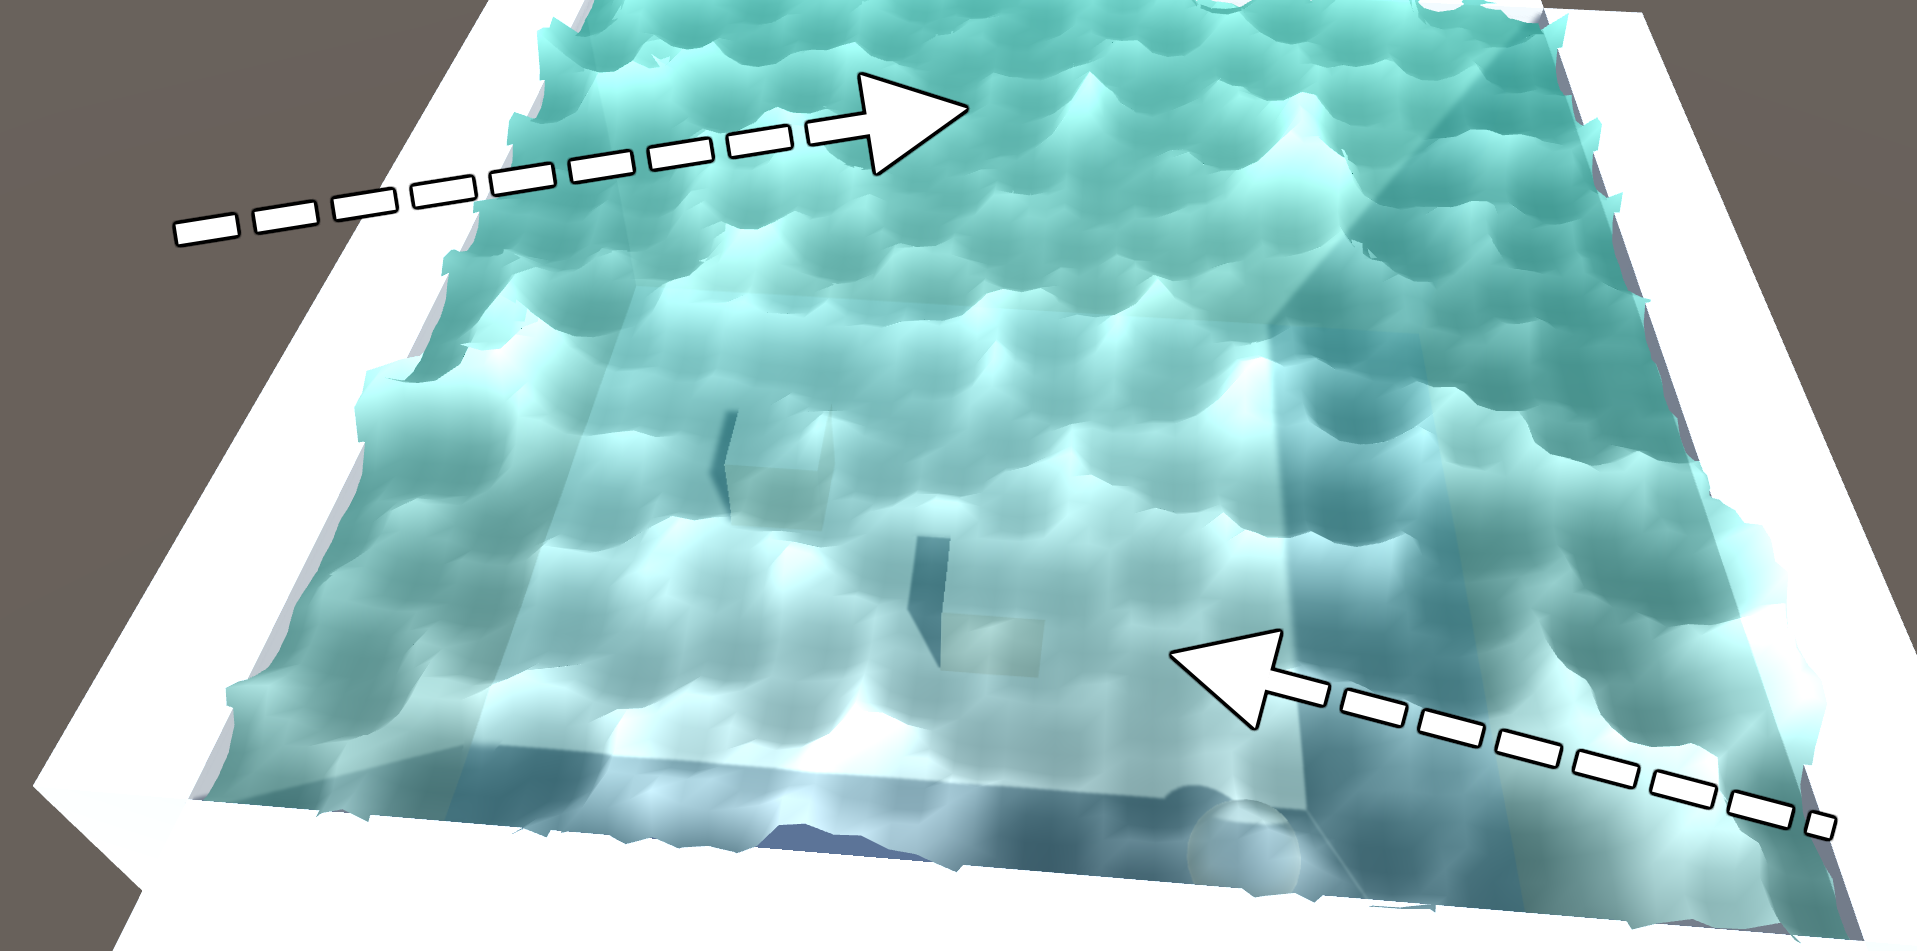
\includegraphics[width=\textwidth]{img/shader_4}
    \caption{Shader}
    \label{fig:shader_4}
\end{figure}

\begin{figure}[H]
    \centering
    \lstinputlisting[firstline=90, lastline=101]{img/voronoi.shader}
    \caption{Voronoi - code implementation in object space}
    \label{fig:voronoi_shader}
\end{figure}
\autoref{fig:voronoi_shader} shows a code snippet from the voronoi implementation. Usually this is used on 2D textures, but since we want to convert it to 3D space we need to do a 3D grid and not a 2D. This is however not needed on a plane or a mesh that which has the same normal vector across the polygons.\\
This code is a very standard or conventional way of implementing voronoi features, besides the additional for-loop on the z axis.\\

Line 4 to 9 is the core of the function, serving to grab the neighbouring grid to later use as an offset. The \texttt{pointt} variable will then hold a random position and have that position modified by time and arbitrary numbers.\\The distance difference will then be calculated and used for colouring the cell or grid square, compared to other points in neighbouring grid cells.

\section{Discussion}
\label{sec:discussion}


\section{Conclusion}
\label{sec:conclusion}



\newpage
\section{Bibliography}
\printbibliography


\end{document}

